\subsection{Menu}

\subsubsection{Gedrag}
Om de gebruiker feedback te geven in welk gedeelte van het menu de wekker zit wordt dat laten zien op het LCD. Het eerste deel wat het subblok \emph{menu} doet, is aangeven wat er op het LCD geschreven moet worden wat er aangepast moet worden. Het tweede deel is een streep zetten onder het deel wat daadwerkelijk aangepast wordt.

\subsubsection{Functionaliteit}
In figuur \ref{fig:FSMmenu} is de FSM te zien van het subblok \emph{menu}. Zolang het menu niet verandert, blijft blijven de uitgangssignalen hetzelfde. Zodra het menu verandert, worden er andere karakters geschreven, welk karakter er geschreven wordt, hangt af van in welk deel van het menu de wekker zit. Zodra het ready-signaal hoog wordt, kan de informatie naar de zender gestuurd worden en als het ready-signaal dan weer laag wordt, is de informatie verstuurd en wordt de nieuwe state weer de steady-state.

\subsubsection{FSM}

\begin{figure}[h!]
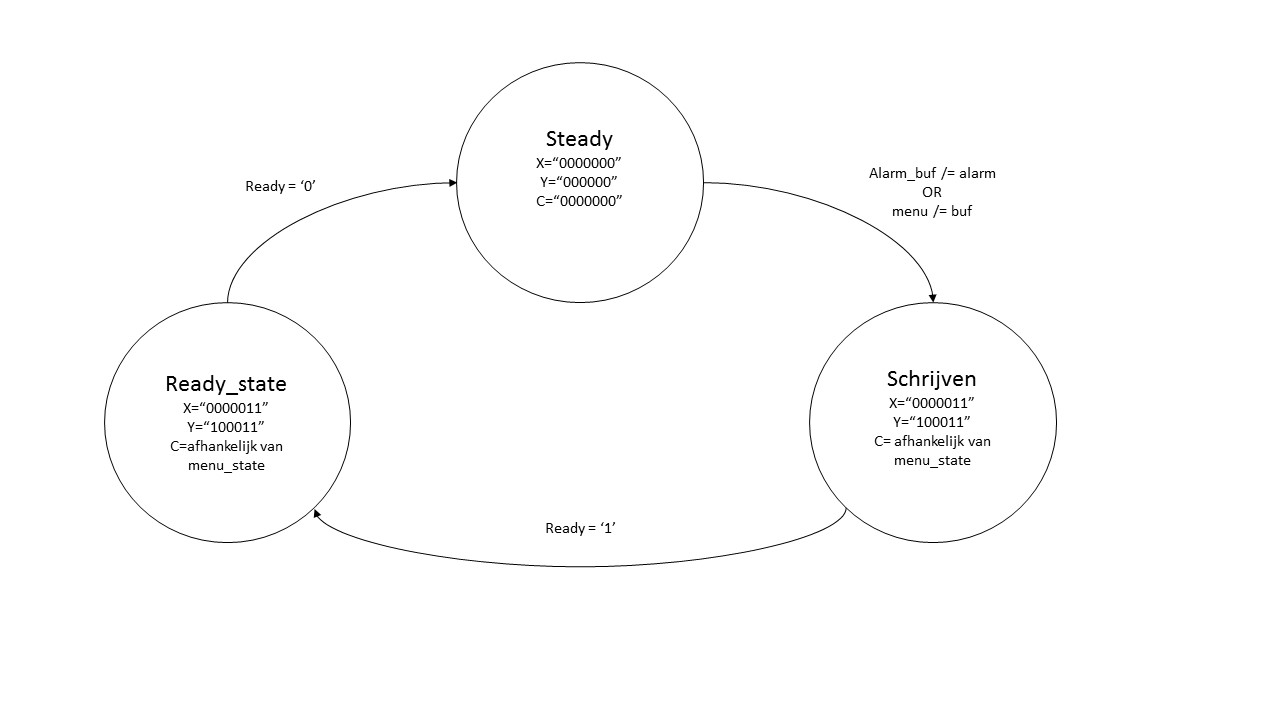
\includegraphics[width=15cm]{verslagschemas/FSMs/menu.jpg}
\caption{FSM van het subblok menu}
\label{fig:FSMmenu}
\end{figure}


\subsubsection{VHDL code}
De VHDL-code van het menu staat in appendix \ref{code:ent_menu_scherm}.

\subsubsection{Simulaties}
In appendix \ref{Ap:sim_LCD} is de simulatie van het subblok \emph{menu} te zien.
